% Related Work

\chapter{Related Work and Used Technologies} % Main chapter title

\label{chapter2_bg}
This chapter presents some background for the content of this thesis.

\section{Related Work}

\subsection{Plotly}
Plotly is a popular public data visualizationcloud service provider. Plotly provides community, professional and enterprise data storage, visualization and analytics services to the user.  Excel, CSV and XML data formats are used to upload the data to its cloud servers.  Plotly provides online graphing, analytics, and statistics tools for individuals and collaboration, as well as scientific graphing libraries for Python, R, MATLAB, Perl, Julia, Arduino, and REST.

\subsection{Loopback}
LoopBack is a highly-extensible, open-source Node.js framework which assimilates the best practices of model driven software develpment. LoopBack simplifies and speeds up REST API development. It consists of a library of Node.js modules for connecting web and mobile apps to data sources such as databases and REST APIs, a command line tool, and client-SDKs. A loopback application has three components: models that represent business data and behavior, data sources and connectors, and mobile clients.An application interacts with data sources through the LoopBack model API, available locally within Node, remotely over REST, and via native client APIs for iOS, Android, and HTML5. Using the API, apps can query databases, store data, upload files, send emails, create push notifications, register users, and perform other actions provided by data sources.
	Loopback is implemented with many of the technologies we use in this thesis. It uses MDSD as a general practice, data access objects for the communication between database and the REST API, access control list for  authorization and is written in Node.js.

\section{Used Technologies}

\subsection{Javascript}
JavaScript (JS)~\cite{crockford2008javascript}, is a high-level, dynamic, weakly typed, object-based, multi-paradigm, and interpreted programming language. Alongside HTML and CSS, JavaScript is one of the three core technologies of World Wide Web content production. It is used to make webpages interactive and provide online programs, including video games. As a multi-paradigm language, JavaScript supports event-driven, functional, and imperative (including object-oriented and prototype-based) programming styles. Initially only implemented client-side in web browsers, JavaScript engines are now embedded in many other types of host software, including server-side in web servers and databases. The most famous server-side Javascript implementation is Node.js.

\subsubsection{Node.js}
\begin{figure}
	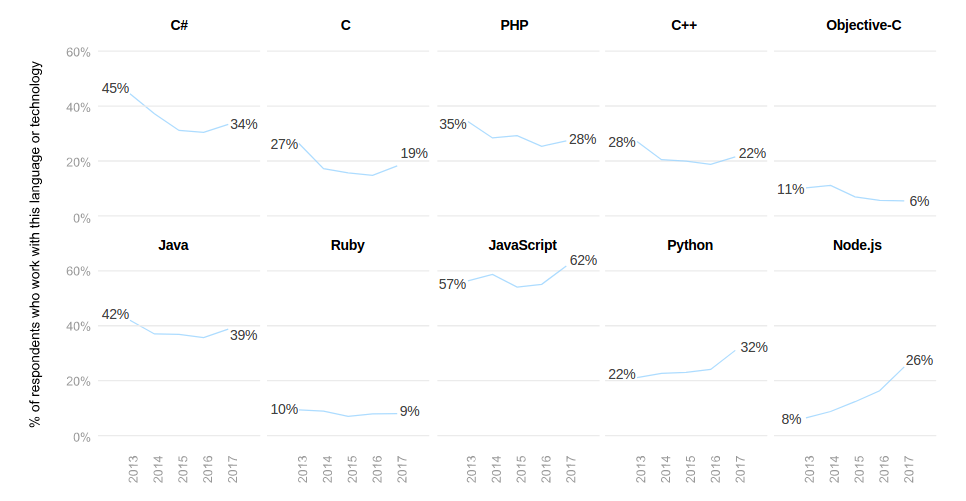
\includegraphics[scale=0.5]{survey17.png}
	\caption{Developers survey for Stack Overflow website in 2017.}
	\label{survey17}
\end{figure}
Node.js~\cite{tilkov2010node} is an open-source, cross-platform JavaScript run-time environment for executing JavaScript code server-side.Node.js provides an event-driven architecture and a non-blocking I/O API designed to optimize application's throughput and scalability for real-time Web applications. It uses Google V8 JavaScript engine to execute code, and a large percentage of the basic modules are written in JavaScript. Node.js contains a built-in library to allow applications to act as a stand-alone Web server. The increasing popularity of Node.js in the last years can be seen in figure~\ref{survey17}.

\subsubsection{Node Package Manager}
Npm~\cite{schlueternode} is a package manager for the JavaScript programming language. It is the default package manager for the JavaScript runtime environment Node.js. It consists of a command line client, also called npm, and an online database of public packages, called the npm registry. The registry is accessed via the client, and the available packages can be browsed and searched via the npm website. Npm is included as a recommended feature in Node.js installer. Npm consists of a command line client that interacts with a remote registry. It allows users to consume and distribute JavaScript modules that are available on the registry. Packages on the registry are in CommonJS format and include a metadata file in JSON format.

\subsection{NoSQL Database}
A NoSQL (originally referring to "non SQL" or "non relational")[1] database provides a mechanism for storage and retrieval of data that is modeled in means other than the tabular relations used in relational databases.NoSQL databases are increasingly used in big data and real-time web applications.Motivations for this approach include: simplicity of design, simpler "horizontal" scaling to clusters of machines (which is a problem for relational databases), and finer control over availability. The data structures used by NoSQL databases (e.g. key-value, wide column, graph, or document) are different from those used by default in relational databases, making some operations faster in NoSQL. The particular suitability of a given NoSQL database depends on the problem it must solve. Sometimes the data structures used by NoSQL databases are also viewed as "more flexible" than relational database tables.

\subsubsection{MongoDB}
MongoDB is a free and open-source cross-platform document-oriented database program. Classified as a NoSQL database program, MongoDB uses JSON-like documents with schemas.


